\documentclass[titlepage]{article}
\usepackage{array}
\usepackage{enumerate}
\usepackage{graphicx}
\usepackage{listings}
\usepackage{tabularx}

\begin{document}

\author{Stevan Stanisic and Santana Mach}
\title{COMP 8505 - Final Project \\ Rootkit \\ Testing Documents}
\date{Dec 05, 2011}
\maketitle{}

\tableofcontents
\pagebreak

\section{Introduction}

The purpose of this experiment was to see how successful we could be in making a covert channel program that would be difficult to detect by system and network administrators. The extent to which this was possible was somewhat surprising to us using tools like linux's raw sockets and the libpcap library.  As our Testing Data shows, common system monitoring  tools, IDSes, and even packet monitoring are little help.  If you don't know what you're looking for, you're unlikely to find it.

Our general strategy was to hide a very small amount of data in certain marked packets and craft the rest of the packet to look like a legitimate request so as not to arouse suspicion. For testing purposes, our data transfer is reasonably fast, however, in a real world setting a channel of this type would likely be limited to a few packets (and therefore bytes) per minute.

We did have to reduce the scope of our program somewhat as noted in the Covert Channel Discussion section, but for the most part we found the work done in the early planning stages to be a very useful guide.  Given that we were able to follow the design quite closely, building the missing features is something we would like to keep in mind for the future.

\section{Usage Instructions}

Installation is not required, the functionality of the program is controlled by command-line switches, simply copy the binary to a surreptitious location on the target machine and either launch it manually or add it to a startup script.

To compile the program from source, the libpcap and openssl development libraries will be required.  Building the program from source should be possible with any version of GCC that supports at least the gnu99 C standard using the provided makefile.  Note, the makefile will also set the setuid bit on the resulting executable as the program requires elevated priveleges to open raw sockets.

The available command-line flags are:
-c : Use this option to activate Client mode. This should be used on the attacker's machine.
-s : Use this option to activate Server mode. This should be used on the victim machine.
-h : Use this option to see a short version of the program usage instructions.
-i <arg> : Use this option to specify the remote host that the machine will be communicating with. For the Client, this will be the server's IP. For the Server, this will be the Client's IP.
-w <arg> : Use this option to specify the folder to watch for exfiltration. Any files created or modified in this folder will be sent to the client.
-x <arg> : Use this option to specify the covert channel to use. 'u' for UDP source port, 'n' for NTP ref\_id, 'd' for DNS transaction id.

If you wish to change the watch folder, the easiest way to do this remotely is to use the ps utility to find your covert process on the victim machine and then execute 'kill <process id>; ./bkdoor -s -w <path> -i <ip> ... other options'.

\clearpage

\section{Testing Design}

The majority of the testing will be carried out from the server (victim) side as this is where monitoring.
The signature for our rootkit is currently `0xAB' with the data encrypted in the next byte.  The signature
can also be configured at compile time, which will be harder for analysts and IDS to detect.
\\

\begin{tabularx}{\textwidth}{|c|X|X|X|c|}
\hline
\textbf{\#} & \textbf{Description} & \textbf{Tools Used} & \textbf{Expected Result} & \textbf{Pass}\\
\hline
1 & Validate IP \& UDP checksums & bkdoor\newline Wireshark & Checksums are correct in Wireshark & Yes\\
\hline
2 & Backdoor channel via UDP source port. & bkdoor\newline Wireshark & Signature \& \newline encrypted data in the source port. & Yes\\
\hline
3 & Backdoor channel via NTP Ref ID. & bkdoor\newline Wireshark & Signature \& \newline encrypted data in the reference clock id. & Yes\\
\hline
4 & Backdoor channel via DNS ID. & bkdoor\newline Wireshark & Signature \& \newline encrypted data in the transaction id. & Yes\\
\hline
5 & Basic commands & bkdoor & Receive output of commands from server & Yes\\
\hline
6 & Exfiltrate file. & bkdoor\newline echo & File is exfiltrated from the server. & Yes\\
\hline
7 & Changing watch\newline directory. & bkdoor & Execute new server with new watching directory & Yes\\
\hline
8 & Resource Monitoring & htop & Backdoor should be indistinguishable from legitimate processes & Yes\\
\hline
9 & Process Monitoring & ps & Backdoor should be indistinguishable from legitimate processes & Yes\\
\hline
10 & Network Monitoring & snort & Backdoor should not trigger any alerts & Yes\\
\hline
11 & Interface Monitoring & netstat & Backdoor should listening mechanisms should not be visible & Yes\\
\hline
\end{tabularx}

\clearpage

\section{Testing Data}

\subsection{Test \# 1 - Checksums}

\begin{figure}[htb]                                                                       
  \begin{center}
    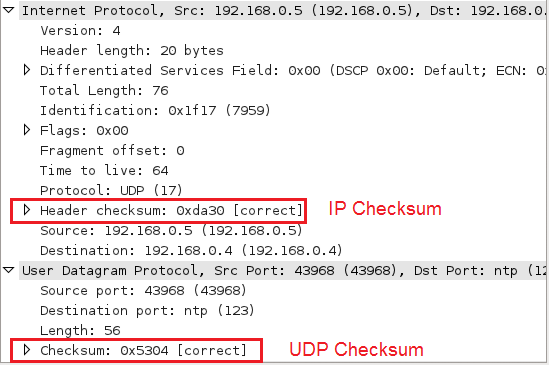
\includegraphics[width=0.9\textwidth]{Pictures/Checksum.png}
  \end{center}
  \caption{IP and UDP Checksums}
  \label{fig:checksums}
\end{figure}

A key to crafting a raw packet is to ensure that there are no warnings to reveal itself.
A good checksum is important for prevent the packet from being dropped or spotted by the IDS.
As shown above, both the IP and UDP checksums are correct.\\

\subsection{Test \# 2 - UDP Channel}

\begin{figure}[htb]                                                                       
  \begin{center}
    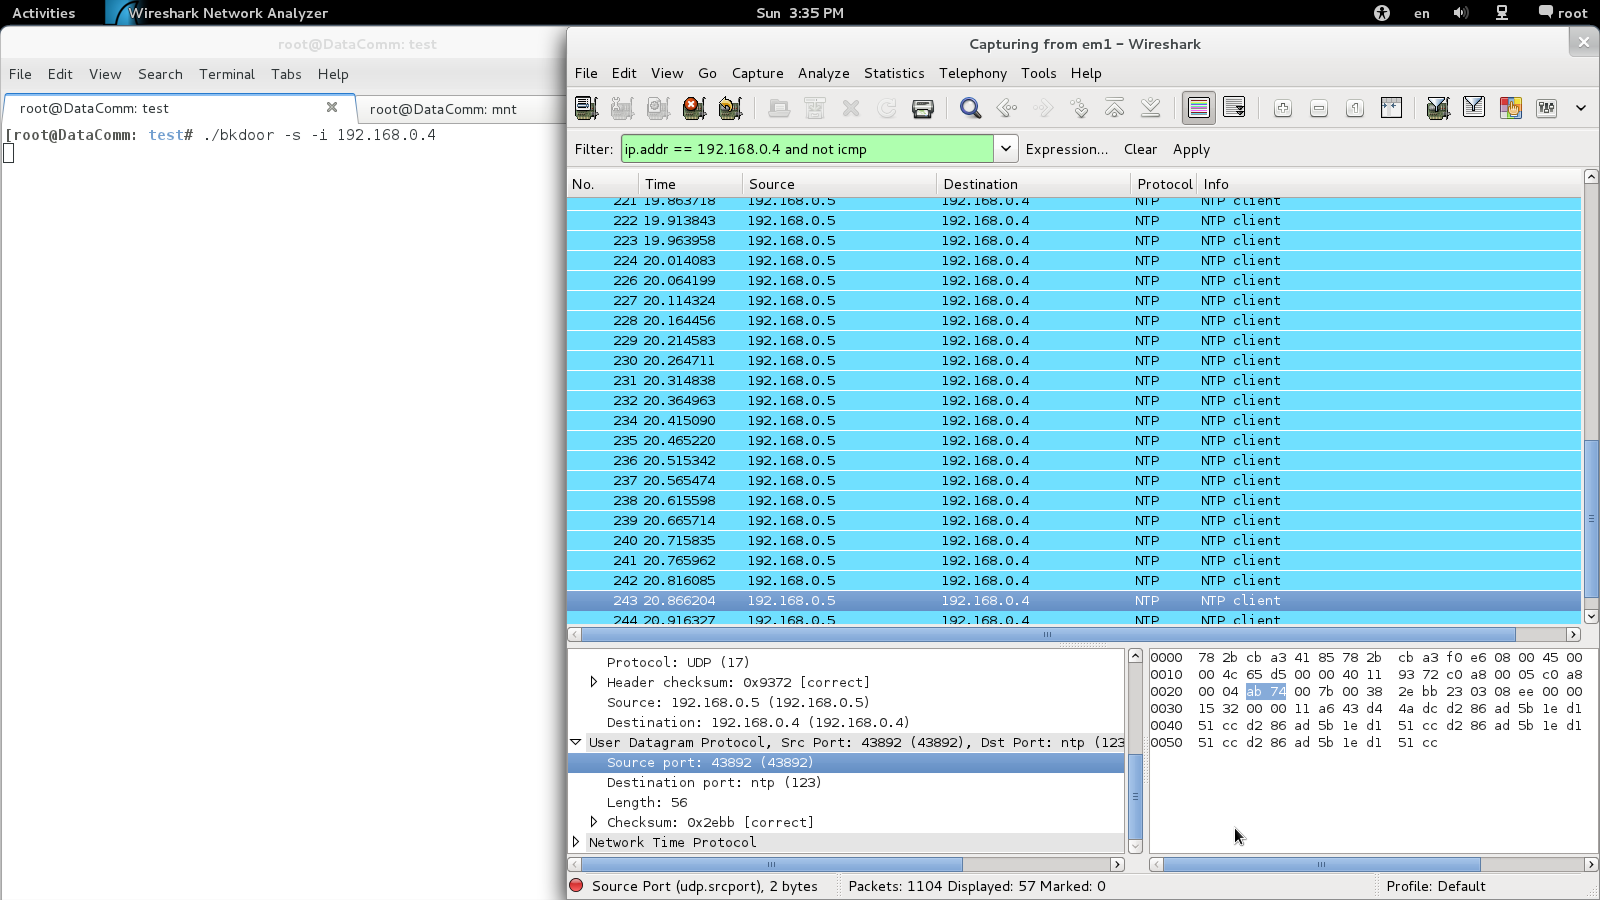
\includegraphics[width=0.9\textwidth]{Pictures/UDP_SIG.png}
  \end{center}
  \caption{UDP Channel Signature}
  \label{fig:udp_sig}
\end{figure}

For the UDP channel, the signature and data are hidden in the source port.  The signature `AB'
can be seen on the first byte with the data encrypted into the second byte.  This results in
a high source port, which is not unusual.  This test was performed using the UDP switch
in the arguments and monitored using Wireshark.

\clearpage

\subsection{Test \# 3 - NTP Channel}

\begin{figure}[htb]                                                                       
  \begin{center}
    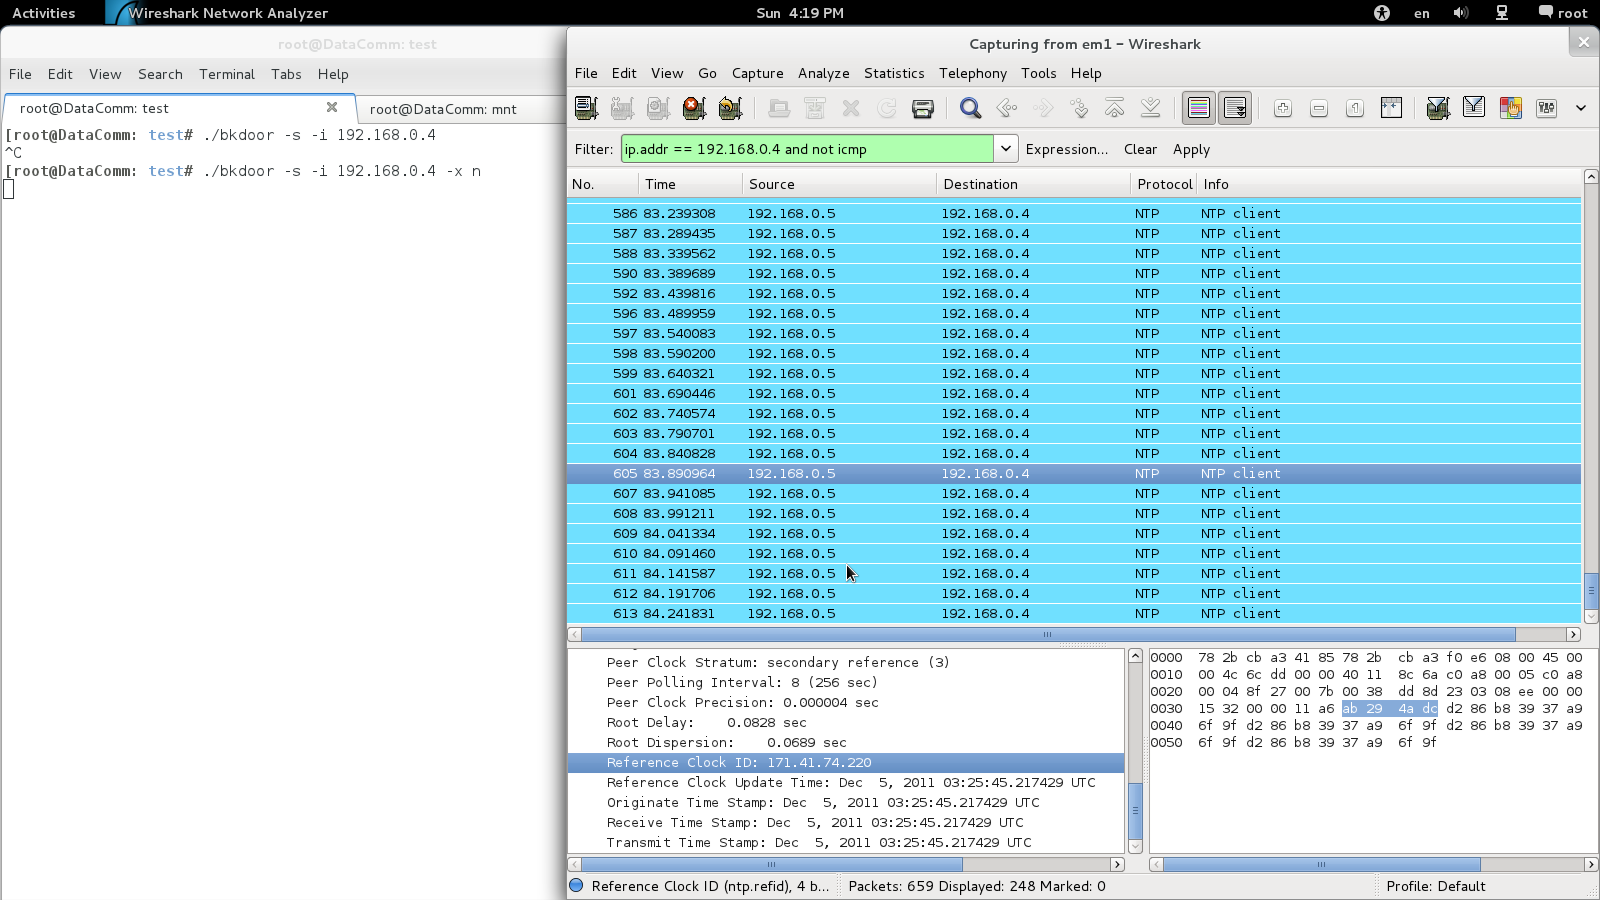
\includegraphics[width=0.9\textwidth]{Pictures/NTP_SIG.png}
  \end{center}
  \caption{NTP Channel Signature}
  \label{fig:ntp_sig}
\end{figure}

The signature and data for the NTP channel is slipped into the Reference Clock ID in the NTP header.
This would be the first two bytes of the ID field.  This test was performed using the NTP switch
in the arguments and monitored using Wireshark.

\subsection{Test \# 4 - DNS Channel}

\begin{figure}[htb]                                                                       
  \begin{center}
    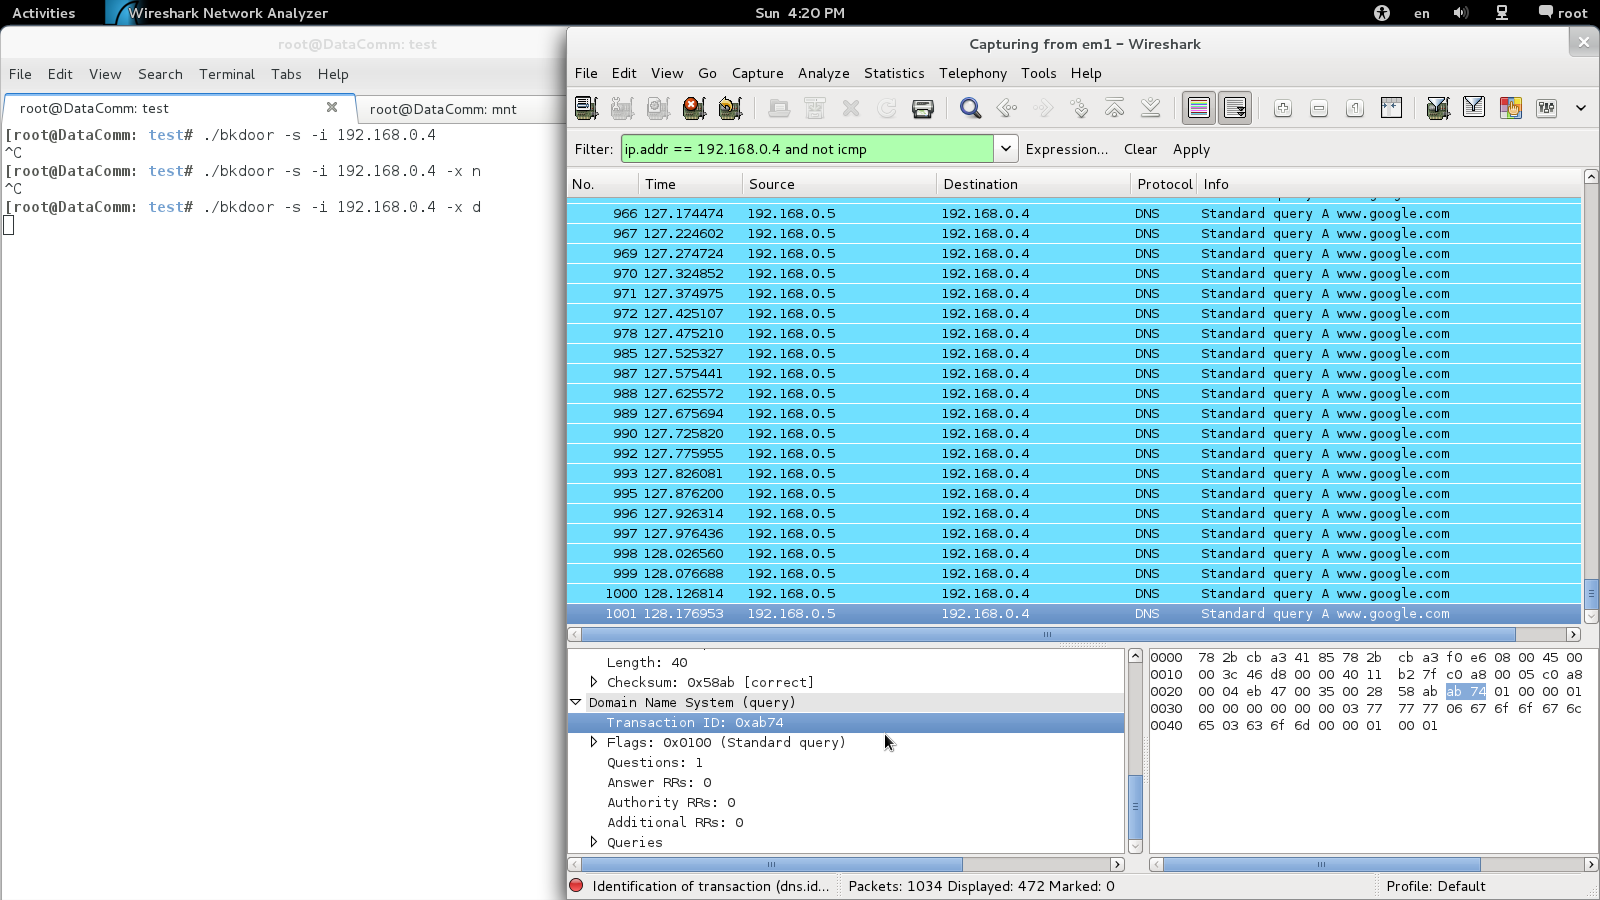
\includegraphics[width=0.9\textwidth]{Pictures/DNS_SIG.png}
  \end{center}
  \caption{DNS Channel Signature}
  \label{fig:dns_sig}
\end{figure}

The field used for the DNS channel is the Transaction ID in the DNS Header.  Similar to the other channels,
the ``AB" signature is placed in the first byte of the field specified.  The transaction id is used to 
match request and reply packets; however, it is not likely monitored.  This test was performed using the NTP
switch in the arguments and monitored using Wireshark.\\

\clearpage

\subsection{Test \# 5 - Basic Commands}

\begin{figure}[htb]                                                                       
  \begin{center}
    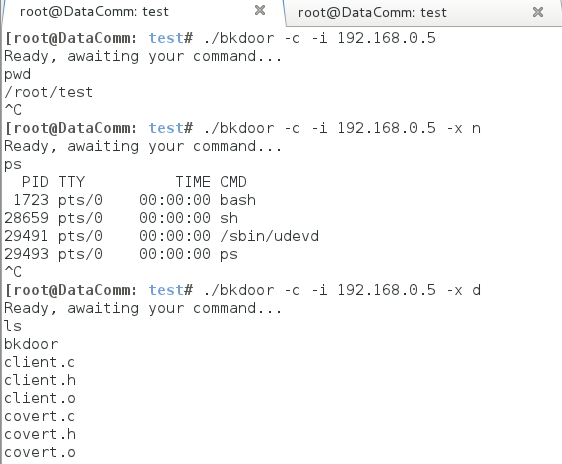
\includegraphics[width=0.9\textwidth]{Pictures/Commands.png}
  \end{center}
  \caption{Output of Commands}
  \label{fig:commands}
\end{figure}

This test shows some of the common commands that are used in a Unix system.  This also demonstrates that
the commands work for all three types of backdoor channel.

\clearpage

\subsection{Test \# 6 - Exfiltration}

\begin{figure}[htb]                                                                       
  \begin{center}
    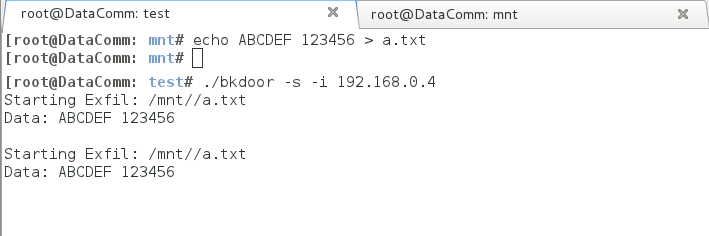
\includegraphics[width=0.9\textwidth]{Pictures/Exfiltration.png}
    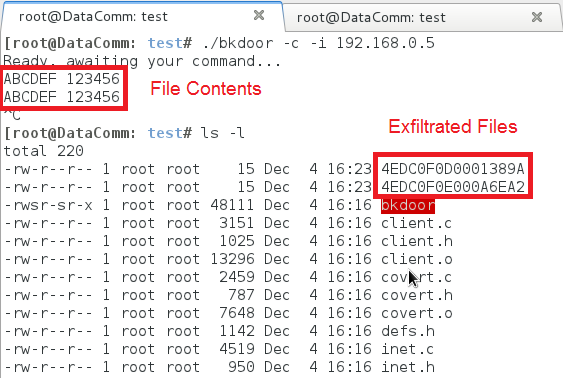
\includegraphics[width=0.9\textwidth]{Pictures/CExfiltration.png}
  \end{center}
  \caption{File Exfiltration}
  \label{fig:exfiltration}
\end{figure}

The default directory for exfiltration is /mnt/ but it can be changed through a switch in
the arguments for the backdoor.  For this test, we used the `echo' tool to create the
file `a.txt' which will notify the watch and exfiltrate the new file.  The client will
print the content to the screen as well as create a file with the current timestamp.\\
\\
We included debug messages for this test to show which file is being exfiltrated; these
messages will not display on the actual program.

\clearpage

\subsection{Test \# 7 - Changing Watch Directory}

\begin{figure}[htb]                                                                       
  \begin{center}
    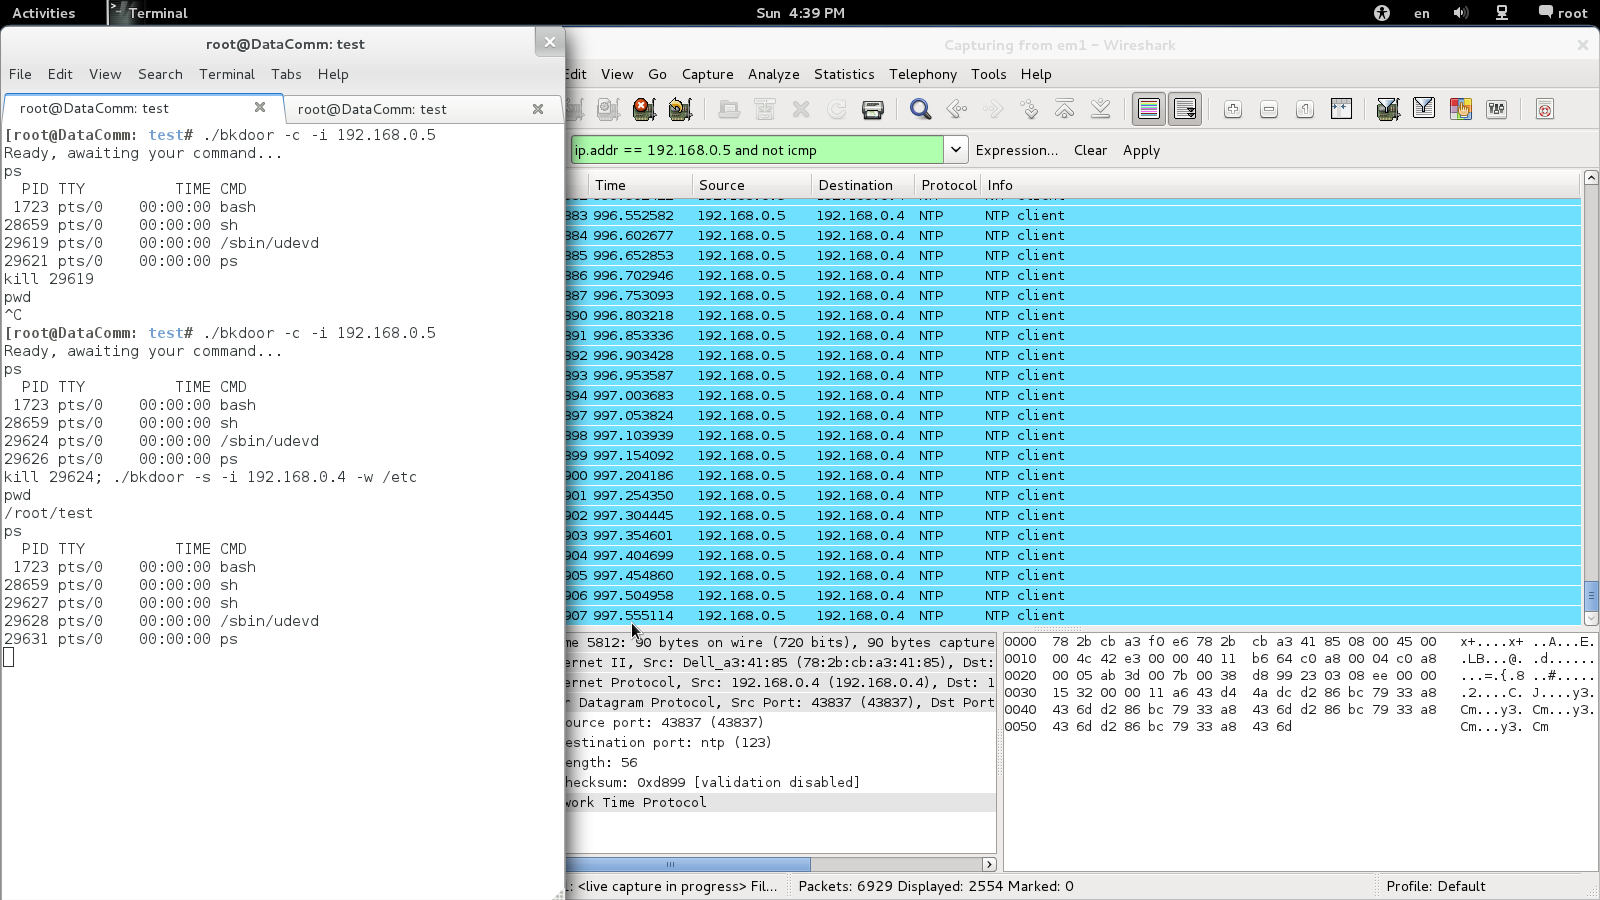
\includegraphics[width=0.9\textwidth]{Pictures/Watch.png}
  \end{center}
  \caption{Example of Watch Directory}
  \label{fig:watch}
\end{figure}

In order to switch the exfiltration watch directory, the client must send the command to
kill the current backdoor and the new one at the same time.  This is because the client
would no longer be able to send commands if there are no servers to receive.  This test
demonstrates the results of both methods.

\clearpage

\subsection{Test \# 8 - Resource Monitoring - htop}

\begin{figure}[htb]                                                                       
  \begin{center}
    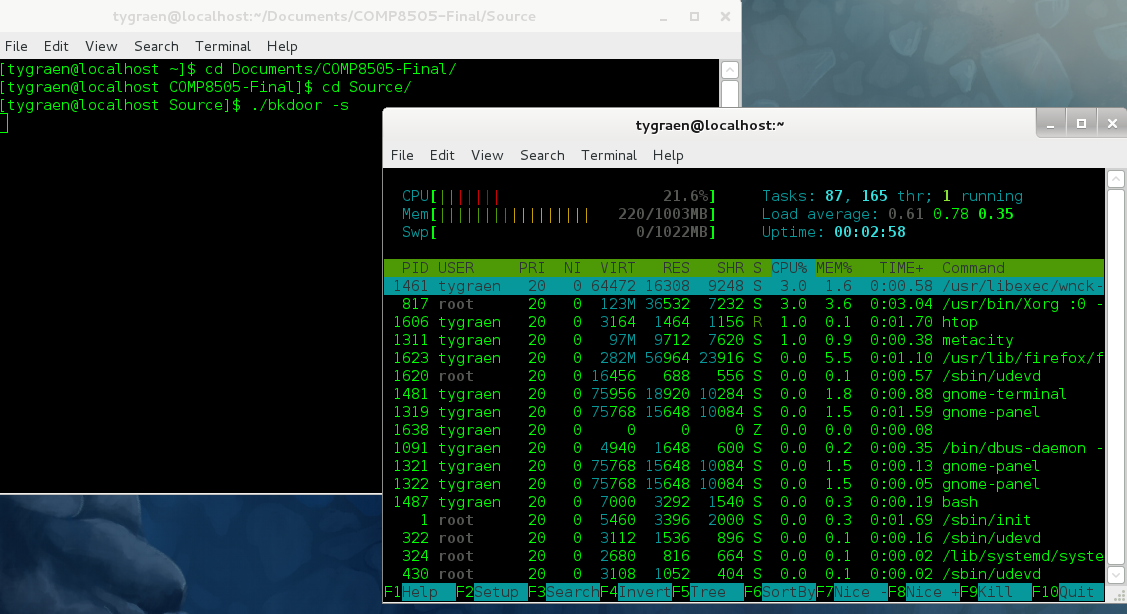
\includegraphics[width=0.9\textwidth]{Pictures/htop.png}
  \end{center}
  \caption{Htop Monitoring}
  \label{fig:htop}
\end{figure}

\clearpage

\subsection{Test \# 9 - Process Monitoring - ps}

\begin{figure}[htb]                                                                       
  \begin{center}
    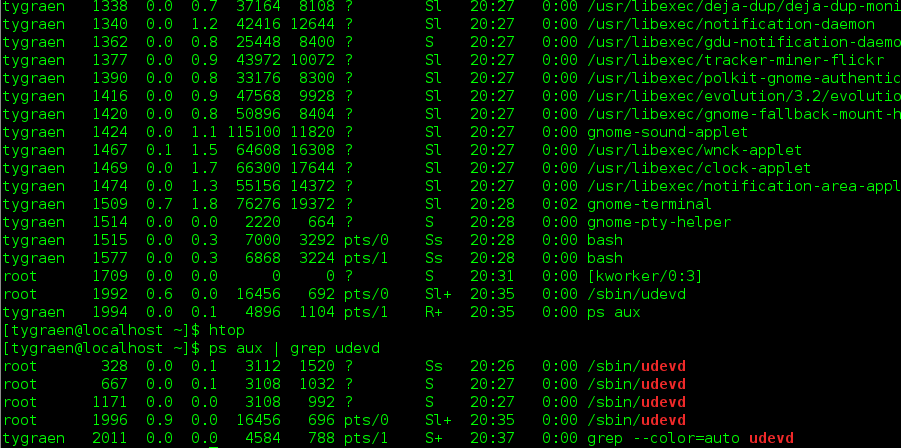
\includegraphics[width=0.9\textwidth]{Pictures/ps.png}
  \end{center}
  \caption{Ps Monitoring}
  \label{fig:ps}
\end{figure}

\clearpage

\subsection{Test \# 10 - Network Monitoring - snort}

\begin{figure}[htb]                                                                       
  \begin{center}
    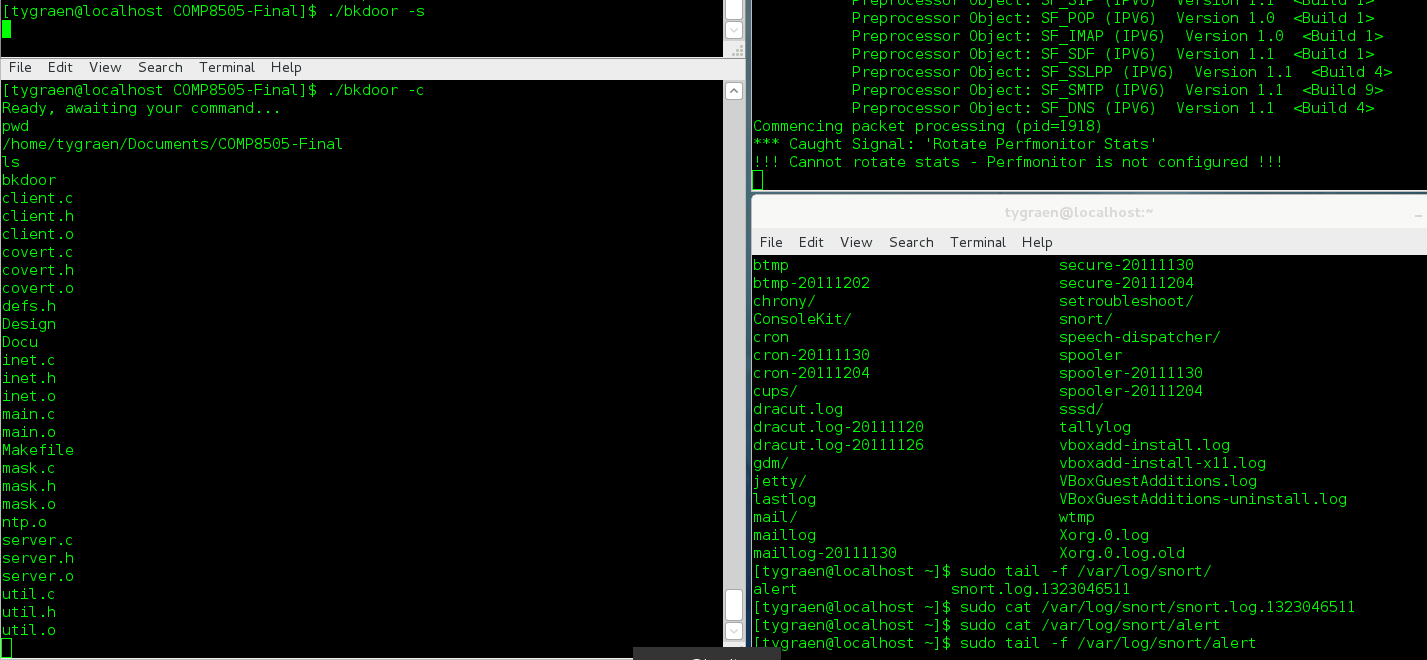
\includegraphics[width=0.9\textwidth]{Pictures/snort.png}
  \end{center}
  \caption{Snort Monitoring}
  \label{fig:snort}
\end{figure}

\clearpage

\subsection{Test \# 11 - Interface Monitoring - netstat}

\begin{figure}[htb]                                                                       
  \begin{center}
    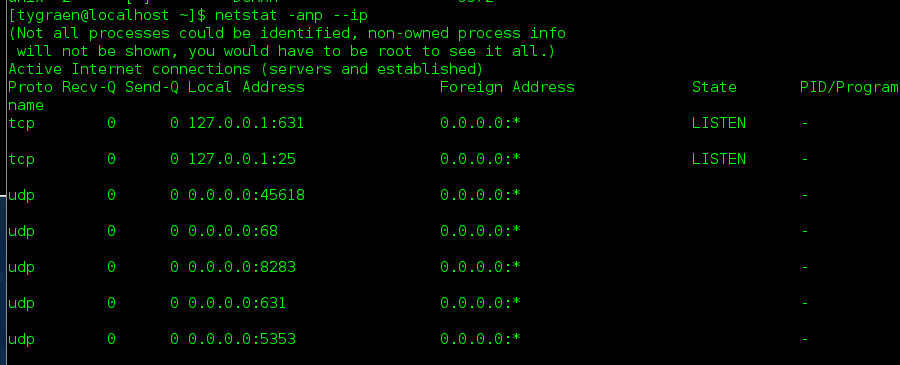
\includegraphics[width=0.9\textwidth]{Pictures/netstat.png}
  \end{center}
  \caption{Netstat Monitoring}
  \label{fig:netstat}
\end{figure}

\clearpage

\section{Covert Channel Discussion}

\subsection{Implementation}

The first thing we should cover is how well we were able to follow the course set out by our Design document.  The specific details of each transmission/frame/packet won't be discussed here as they were already covered in some depth in the Design document. We were able to implement the Transmission level, Frame level and Packet level mechanisms quite easily.  We decided to increase the length of the Signature at the Packet level to 1B and drop the Offset field as our packets go out too slowly to encounter re-ordering.  The Frame level logic made enabling full 64bit DES encryption/decryption quite easy.  We do also include the password check and MD5 hash for data verification as planned at the Transmission level, however, we did not have time to add a reliability layer so it is of limited value. We would not recommend use of this Proof of Concept tool on a highly congested network.

Using libpcap on the Server(victim) was very useful as we didn't have to worry about firewall settings or giving ourselves away to common administrator tools such as netstat or ps (masked executable).  We chose to use a Raw Socket to read packets on the Client (attacker) as it made the program loop a little bit more straightforward and the additional features available through the libpcap library weren't necessary on the client's side.

Regarding covert channel types, we implemented our UDP header and NTP payload covert channel without much in the way of problems.  We decided not to pursue an ICMP based covert channel for two reasons. One, aside from echo requests/responses and destination unreachable messages we don't see much ICMP traffic flowing through most networks. Two, selecting a second application layer-level protocol made sense from a workload perspective as it provided a necessary cover as well as reducing coding effort as we would not have to craft another kind of transport layer packet.  For these reasons we chose to use the DNS payload based for our final covert channel.

\subsection{Defense}

As we saw from the testing section, detecting a cleverly hidden backdoor is nearly impossible.  The fact that the packets look like perfectly legitimate requests certainly does not make a network administrators job easier. If we decided to track all traffic types, we could look for an increase in a certain request type, but this isn't an ideal solution. Simply slowing down transmission should make it stand out less or the attacker could simply switch between signatures; this could also potentially cause a large number of false positives as legitimate usage patterns change.

A cleverly hidden backdoor isn't impossible to detect on a compromised system, but monitoring a large number of systems with enough attention to detail could potentially be very time consuming.  The first thing an administrator should look for are setuid executables, there should be a very small number of these, if any on a given system.  We've already seen that the netstat, top and ps utilities are unable to give us any useful information. 

There are a couple of things we can do to increase our chances of detecting this type of activity at the sys-admin level. We can use log-monitoring applications to hopefully detect the initial intrusion; if this is an inside job by a legitimate user, this may be difficult.  If we have a relatively static configuration, we can audit all binary executables using MD5 or SHA1 hashes. If users are required to install or download things regularly, this may be too time-consuming in practice.

\section{Conclusion}

As mentioned before, we knew it would be difficult to detect a covert channel, but we were surprised by exactly how much. Once the data is encrypted, there is very little to give the backdoor away, especially if the machine being used commonly receives the particular traffic type which is being used as a cover.

Now that the experiment is finished, looking forward we would like to think about adding reliability/timeout extensions sometime in the future.  The other point mentioned in our Design document is that we would like to look at embedding the backdoor in a kernel module. The disadvantage to that approach is that it becomes much more tailored to a single machine/kernel version, but it would be even more difficult to detect and gives us the luxury of not having to worry about priveleges and permissions.

Another topic that would be interesting to look into would be if it is possible to use statistical methods to detect covert channels or if network traffic on a real-world network would cause too many false positives.  It likely depends more on the volume of data the attacker is trying to steal and how patient they are than anything else.  The slower the transfer, the more it fades into the background noise that is always present on a given network.

\end{document}
